\documentclass[UTF8, 11pt, a4paper]{article}
\usepackage[cm]{sfmath}
\usepackage{tabularx}
\def\arraystretch{1.3}
\usepackage[a4paper, top=3.18cm,bottom=3.81cm,left=2.54cm,right=2.54cm]{geometry}
\usepackage{indentfirst}
\setlength{\parskip}{6pt}
\XeTeXlinebreaklocale "zh"
\usepackage{graphicx}
\usepackage[normalem]{ulem}

\usepackage{fontspec}
\setmainfont{思源黑体}
\SetSymbolFont{largesymbols}{normal}{OMX}{iwona}{m}{n}
\setmonofont{Source Code Pro}

\begin{document}
\section*{举步维艰 / Stumbler \makebox[2.5em]{} \small{「STUMBLER」}}
Gravitus 是一位资深 osu! 玩家。%
自从最近入手了一个无限大的显示器,这个游戏的谱面真是变得越来越有趣了……

这天 Gravitus 正在研究一张谱面的图形形状。这个二维平面上的形状由许多打击物件组成,%
每个物件可以是圆圈 (Circle) 或者滑条 (Slider) 中的一种。其中滑条是%
由两端的圆和联结圆心的宽度等于圆直径的矩形组成的一种“药丸形”的物体,具体可参考下图。

\begin{figure}[h]\centering
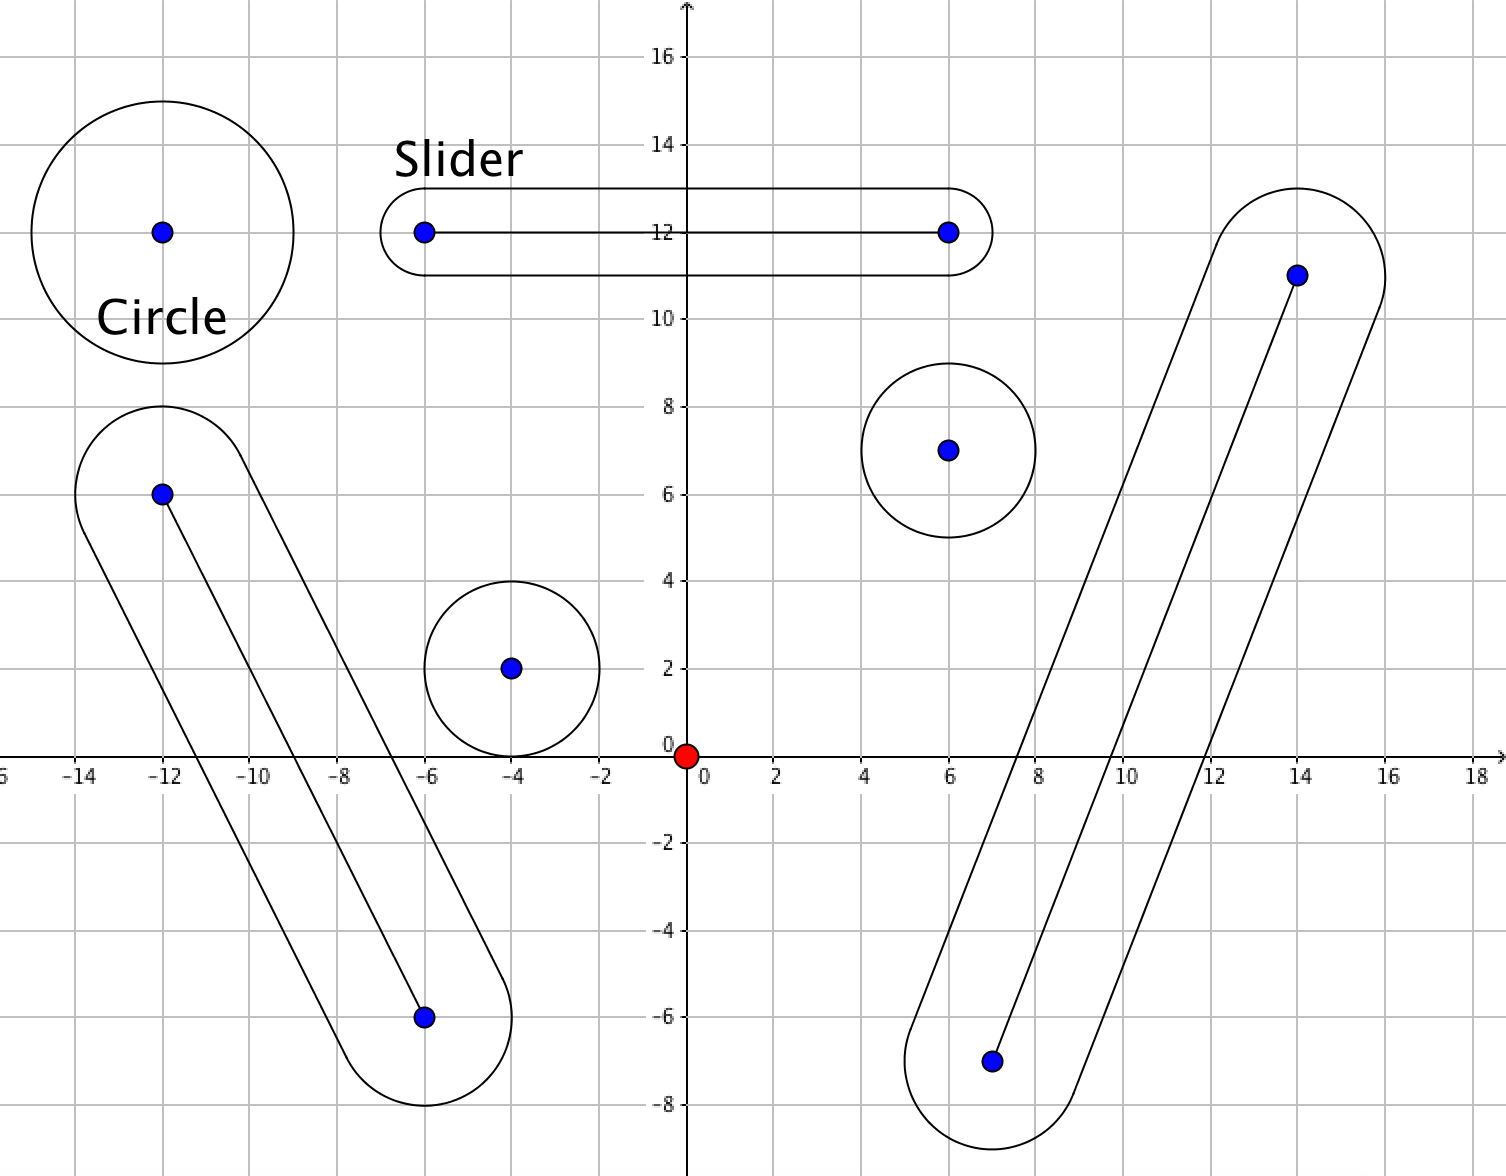
\includegraphics[scale=0.22]{desc.png}
\end{figure}

当然这个谱面是无法做到全连的 ←\_←。尽管如此,Gravitus 还是决定体验一把。%
屏幕上突然同时出现了很多很多的打击物件,而此时 Gravitus 的鼠标停留在屏幕中央 $(0, 0)$ %
处。Gravitus 决定等概率随机选择一个 $[-\pi, +\pi)$ 中的角度 $\theta$,然后将鼠标沿着%
与横坐标轴正半轴夹角 $\theta$ 的射线方向永不停歇地移动鼠标(毕竟显示器是无限大的)。

盯着谱面发了半天呆之后,Gravitus 发现,鼠标的初始位置 $(0, 0)$%
\uwave{不在任何一个物件的内部}  \uwave{或边缘上}。

Gravitus 非常想让自己的鼠标在移动的路线上有且仅有一个打击物件。%
打击物件在鼠标移动的路线上,当且仅当打击物件的闭合图形与上述射线有公共点。%
又一次盯着谱面发了半天呆之后,Gravitus 知道了这个愿望实现的概率。%
你是不是可以在 Gravitus 知道你不知道这个值之前先知道这个值呢?

\subsection*{任务}
对于给定的谱面描述(保证满足上述条件,不必进行检查),%
计算有且仅有一个打击物件在 Gravitus 的鼠标移动路线上的概率。

\subsection*{输入 \makebox[0.5em]{} \small{stumbler.in}}
\begin{itemize}
    \item 第 $1$ 行:两个整数 $N_\mathrm{C}$ 和 $N_\mathrm{S}$,分别表示圆圈和滑条的数量。
    \item 第 $2 \sim N_\mathrm{C} + 1$ 行:%
        每行三个整数 $X$、$Y$、$R$,依次描述一个圆圈的圆心横纵坐标和半径长度。
    \item 第 $N_\mathrm{C} + 2 \sim N_\mathrm{C} + N_\mathrm{S} + 1$ 行:%
        每行五个整数 $X_1$、$Y_1$、$X_2$、$Y_2$、$R$,依次描述一个滑条两端圆心的横纵坐标和%
        圆的半径长度。保证相对于原点 $(0, 0)$,点 $(X_2, Y_2)$ 在点 $(X_1, Y_1)$ 的逆时针方向。
\end{itemize}

\subsection*{输出 \makebox[0.5em]{} \small{stumbler.out}}
\begin{itemize}
    \item 第 $1$ 行:一个正实数 $P$ 表示所求概率,用十进制直接表示%
        (不保证科学计数法能够正常识别),精度任意。
\end{itemize}

在评分时,设陪审团给出的答案为 $P^*$,那么当 $P$ 与 $P^*$ 的绝对误差不超过 %
$10^{-6}$,即 $|P^* - P| \leq 10^{-6}$ 时,答案被判定为正确。

\subsection*{样例}
\begin{table}[h]\centering
\begin{tabularx}{0.8 \textwidth}{|X|X|}
\hline
\texttt{\textbf{stumbler1.in}} & \texttt{\textbf{stumbler1.out}} \\ \hline
{\ttfamily
3 3\newline
6 7 2\newline
-4 2 2\newline
-12 12 3\newline
6 12 -6 12 1\newline
-12 6 -6 -6 2\newline
7 -7 14 11 2
} & {\ttfamily
0.6324337557
}
\\ \hline
\end{tabularx}\end{table}

样例一满足子任务 3 的限制,对应的图形与题目描述中的图形相同。

\begin{table}[h]\centering
\begin{tabularx}{0.8 \textwidth}{|X|X|}
\hline
\texttt{\textbf{stumbler2.in}} & \texttt{\textbf{stumbler2.out}} \\ \hline
{\ttfamily
6 0\newline
0 10 5\newline
6 0 3\newline
-6 0 4\newline
-8 9 4\newline
-6 -8 2\newline
5 -7 2
} & {\ttfamily
0.6964586029
}
\\ \hline
\end{tabularx}\end{table}

样例二对应的图形如下图所示。
\begin{figure}[h]\centering
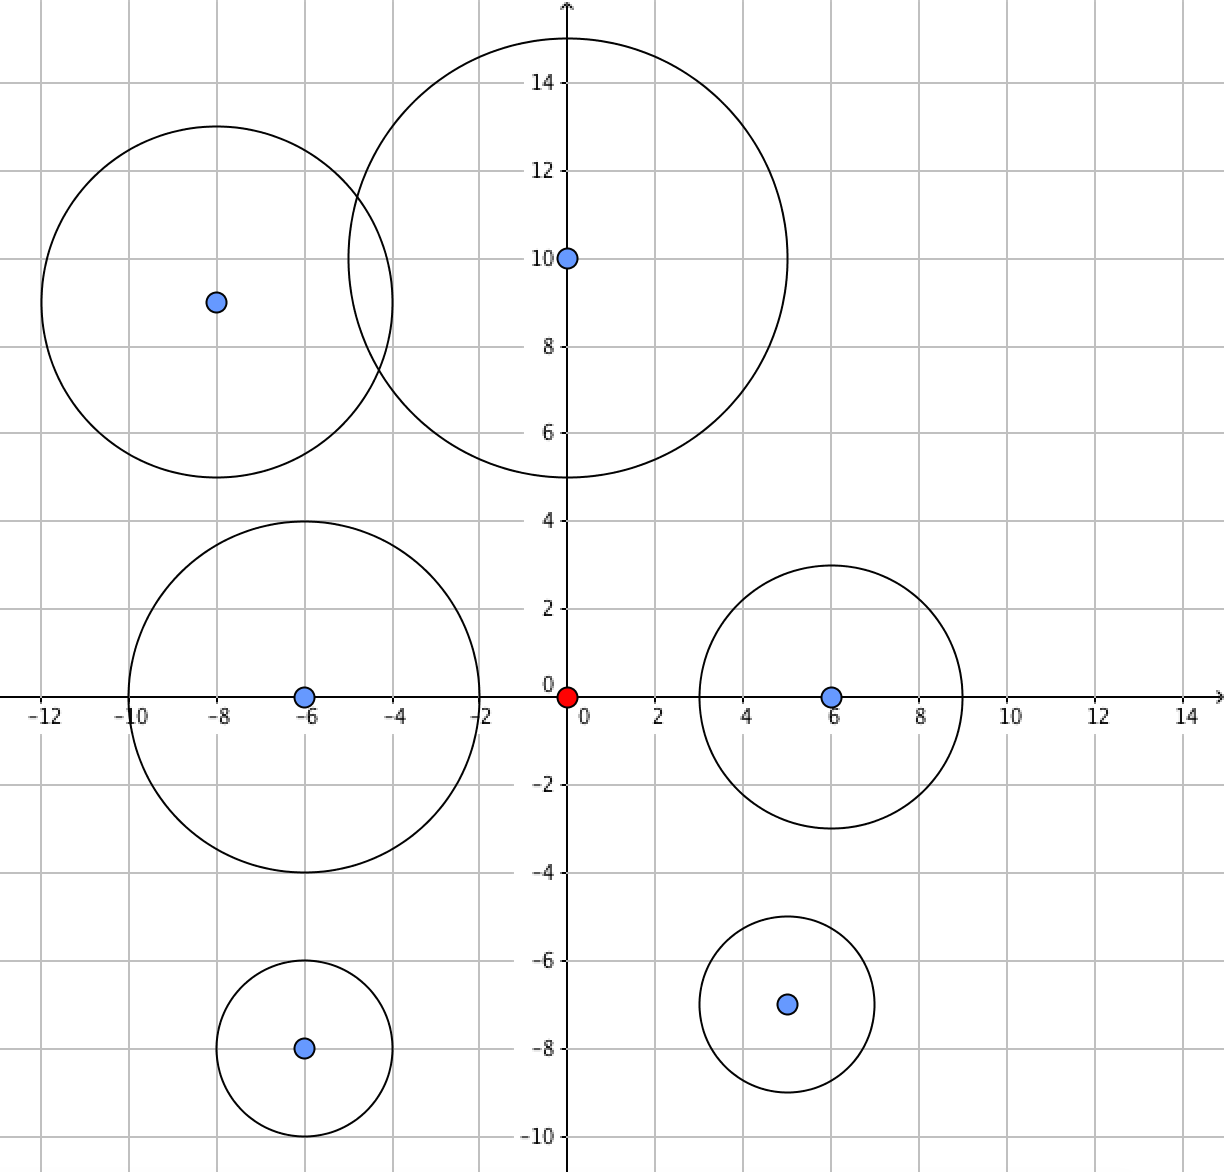
\includegraphics[scale=0.22]{s2.png}
\end{figure}

\subsection*{数据规模与约定}
对于所有子任务,有 $0 \leq N_\mathrm{C}, N_\mathrm{S} \leq 50\,000$,%
所有坐标的绝对值不超过 $10^5$。
\subsubsection*{子任务 1 “Easy” (10 pts)}
\begin{itemize}
    \item $N_\mathrm{C} \leq 1\,000$。
    \item $N_\mathrm{S} = 0$。
    \item 不存在一条从原点出发的射线与多于一个打击物件有公共点。
\end{itemize}
\subsubsection*{子任务 2 “Normal” (23 pts)}
\begin{itemize}
    \item 不存在一条从原点出发的射线与多于一个打击物件有公共点。
\end{itemize}
\subsubsection*{子任务 3 “Hard” (34 pts)}
\begin{itemize}
    \item $N_\mathrm{C}, N_\mathrm{S} \leq 1\,000$。
\end{itemize}
\subsubsection*{子任务 4 “Insane” (16 pts)}
\begin{itemize}
    \item 存在一个点 $P_0$ 使得每一个打击物件都满足 $P_0$ 在它的内部或边缘。
\end{itemize}
\subsubsection*{子任务 5 “Another” (17 pts)}
    没有任何附加限制。

\subsection*{限制}
\begin{itemize}
\item 时间:2.0 秒
\item 内存:1.0 GiB
\end{itemize}

\begin{figure}[h]\centering

\includegraphics[scale=0.55]{stumbler.png}
\end{figure}

\end{document}

